\chapter{ヒッグス粒子を解き明かす}

\lectureoverview{ヒッグス機構は、その構成要素が必要となる順序に従って理解するのが最もよい。まず量子化された運動と場から始め、ありふれた椀をメキシカンハット型ポテンシャルに変え、そこで生じる凝縮体を用いて、なぜフェルミオンと弱ゲージボソンが質量をもちうるのかを理解する。その後になって初めて、物理的なヒッグス粒子をその凝縮体の動径方向の振動として同定し、2012年にその発見をもたらした生成と崩壊の過程を追う。}

\section{見出しの背後にある機構}

$125\,\mathrm{GeV}$付近での新粒子の発見は、当然ながら興奮すべきものであったが、興奮はまだ理解ではない。有用な問いは、ヒッグスが重要かどうかでも、それを宇宙の起源と修辞的に結びつけられるかどうかでもない。有用な問いはもっと狭い。すなわち、この現象の具体的な仕組みは何であり、なぜ標準模型がそれを必要としたのか、である。

この名称にも簡単な限定を付しておく価値がある。ピーター・ヒッグスはこの物理を特定した複数の人物の一人であり、Fran\c{c}ois エングレールとロバート・ブラウトは独立に中心となる着想に到達した。したがって \emph{Brout--Englert--Higgs 機構} という表現のほうが歴史をより忠実に記録しているが、以下ではより短い名称を用いる。

説明はいくつかのモジュールからなる。まず量子力学の二つの基本的な事実と、古典場の理論からの一つのアイデアが必要である。次に、最低エネルギー状態が非零の場を含む真空が必要である。その後で標準模型の粒子を数え上げ、理論の裸の版がなぜ関連する粒子を質量ゼロのままにするのかを見ることができる。ヒッグス粒子そのものは終わり近くになって初めて現れる。それは機構の全体ではなく、機構が整った後に残る一つの特定の振動である。

\section{二つの量子的事実と一つの場}

第一の量子的事実は量子化である。角運動量は、離散的な単位で現れるため、きれいな原型である。
\begin{equation}
L=n\hbar,
\qquad
n=0,\pm1,\pm2,\ldots .
\end{equation}
半整数の角運動量も生じるが、当面の議論はそれに依存しない。重要なのは、連続的に変化する古典的運動が量子状態の梯子になるということである。

第二の事実は不確定性原理である。可能な真空の連続的な円が現れるまで、それは保留する。そのときそれは、真空を、一つの鋭く指定された点に静止して座る小さな古典的な球として扱うことを妨げるであろう。

これら二つの量子的事実の間に、場という古典的な概念がある。場は、空間と時間の各点に量を割り当てる。電場、磁場、重力場はよく知られた例である。ある領域は、空に見えてもなお場を含みうる。観測者から遠く離れ、どちらも見えない場所にある二枚の帯電板を想像しよう。それらの間のほぼ一様な電場は、それでも局所的に実在する。したがって``空の空間''は、必ずしも``すべての場がゼロに等しい''ことを意味しない。それは、場が利用可能な最低エネルギーの状態を占めていることを意味する。

場のエネルギーが一つの値で最小になり、場が変位すると増大するとしよう。場が乱されれば、それは最小値のまわりで振動する。量子力学はそれらの振動を量子化し、個々の量子は粒子である。これが講義全体で必要となる場の理論の辞書である。
\begin{equation}
\text{particle}
\quad\longleftrightarrow\quad
\text{quantum of a field vibration}.
\end{equation}

\section{場の空間における椀}

一つの実数の場の成分$\phi$に対して、最も単純なエネルギーの地形は椀である。
\begin{equation}
V(\phi)=\frac{1}{2}m^{2}\phi^{2}.
\end{equation}
椀の底は$\phi=0$にある。底のまわりの小さな振動は確定した振動数をもち、その量子は質量$m$の粒子として振る舞う。

次に、単一の場を二つの成分$(\phi_1,\phi_2)$に置き換える。エネルギーはこの内部平面における半径のみに依存しうる。
\begin{equation}
r^{2}=\phi_1^{2}+\phi_2^{2},
\qquad
V=V(r).
\end{equation}
これは\emph{場の空間}上の椀であり、通常の空間におけるくぼみではない。対$(\phi_1,\phi_2)$を回転させてもエネルギーは変わらない。講義で用いられる帽子は同じ対称性を可視化する。すなわち、その軸のまわりに回しても、それは依然として同じに見える。

\begin{figure}[tbp]
\centering
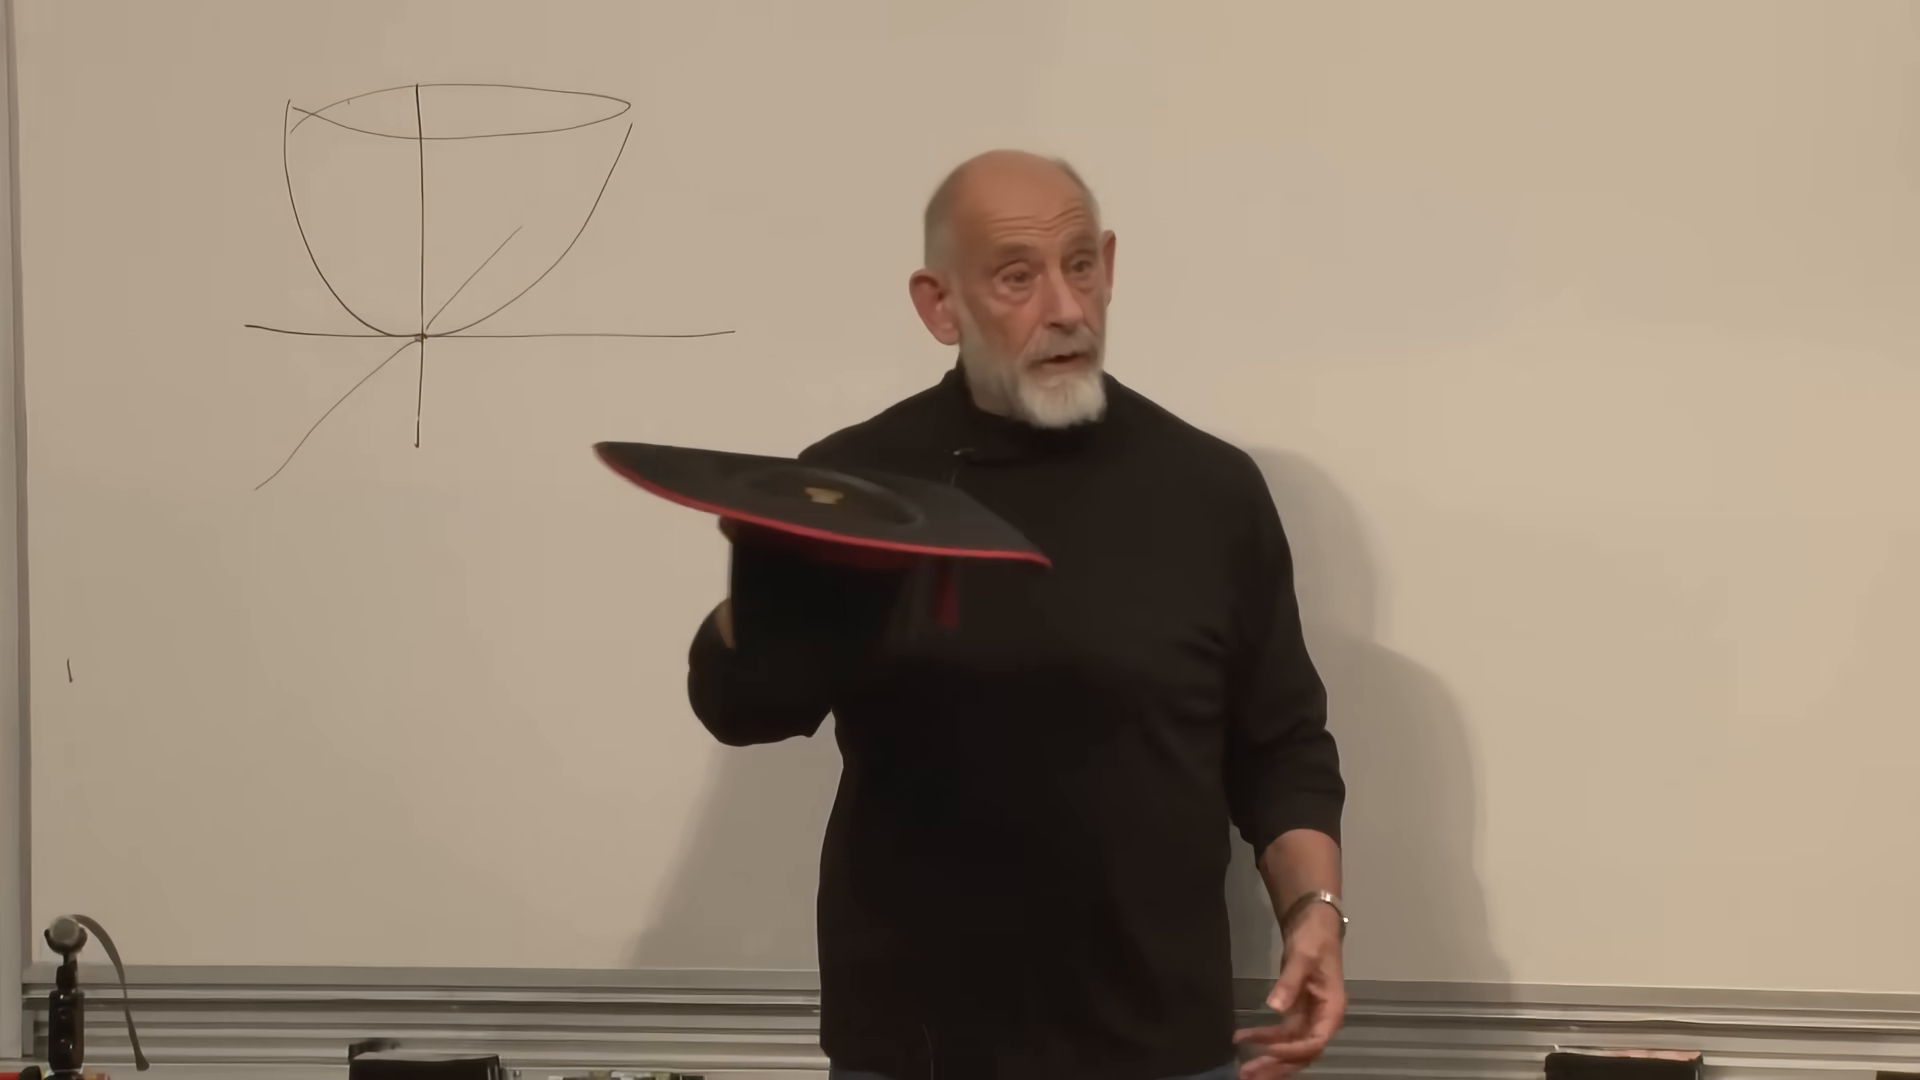
\includegraphics[width=0.95\textwidth]{lecture_144_figure_02.png}
\caption{場の空間における回転対称性を具体的に感じさせるために用いられる、通常の対称な椀と物理的な帽子。}
\lectureframe{00:10:02}
\end{figure}

場が動くと、この類推は単なる幾何学ではなくなる。場を中心から変位させ、鉢の周りを循環させる。この循環は場の空間における角運動量を運ぶ。これは実験室で物体が回転するときの角運動量ではなく、内部角運動量である。量子化されると、保存電荷の模型を与える。
\begin{equation}
Q=nq_0,
\qquad
n\in\mathbb{Z}.
\end{equation}
この式は模式的なものである。中心となる物理的考え方は、荷電場の励起は内部平面内の回転として描けるということである。正電荷と負電荷は反対向きの回転に対応し、回転がないことは電荷ゼロに対応する。

\section{帽子をひっくり返す}

普通の鉢には最低点が一つしかない。ヒッグス物理は帽子をひっくり返すところから始まる。中心はもはや不安定であり、一方、円形の溝全体が同じ最小エネルギーをもつ。標準的な数学的実現は
\begin{equation}
V(\phi_1,\phi_2)
=
\lambda
\left(
  \phi_1^{2}+\phi_2^{2}-v^{2}
\right)^{2},
\qquad \lambda>0,
\end{equation}
であり、その最小値は
\begin{equation}
\phi_1^{2}+\phi_2^{2}=v^{2}.
\end{equation}
を満たす。
\editorialnote{この明示的な四次ポテンシャルは、講義で描かれたメキシカンハット幾何学の標準的な解析的完成であり、板書の式を書き写したものではない。}

\begin{figure}[tbp]
\centering
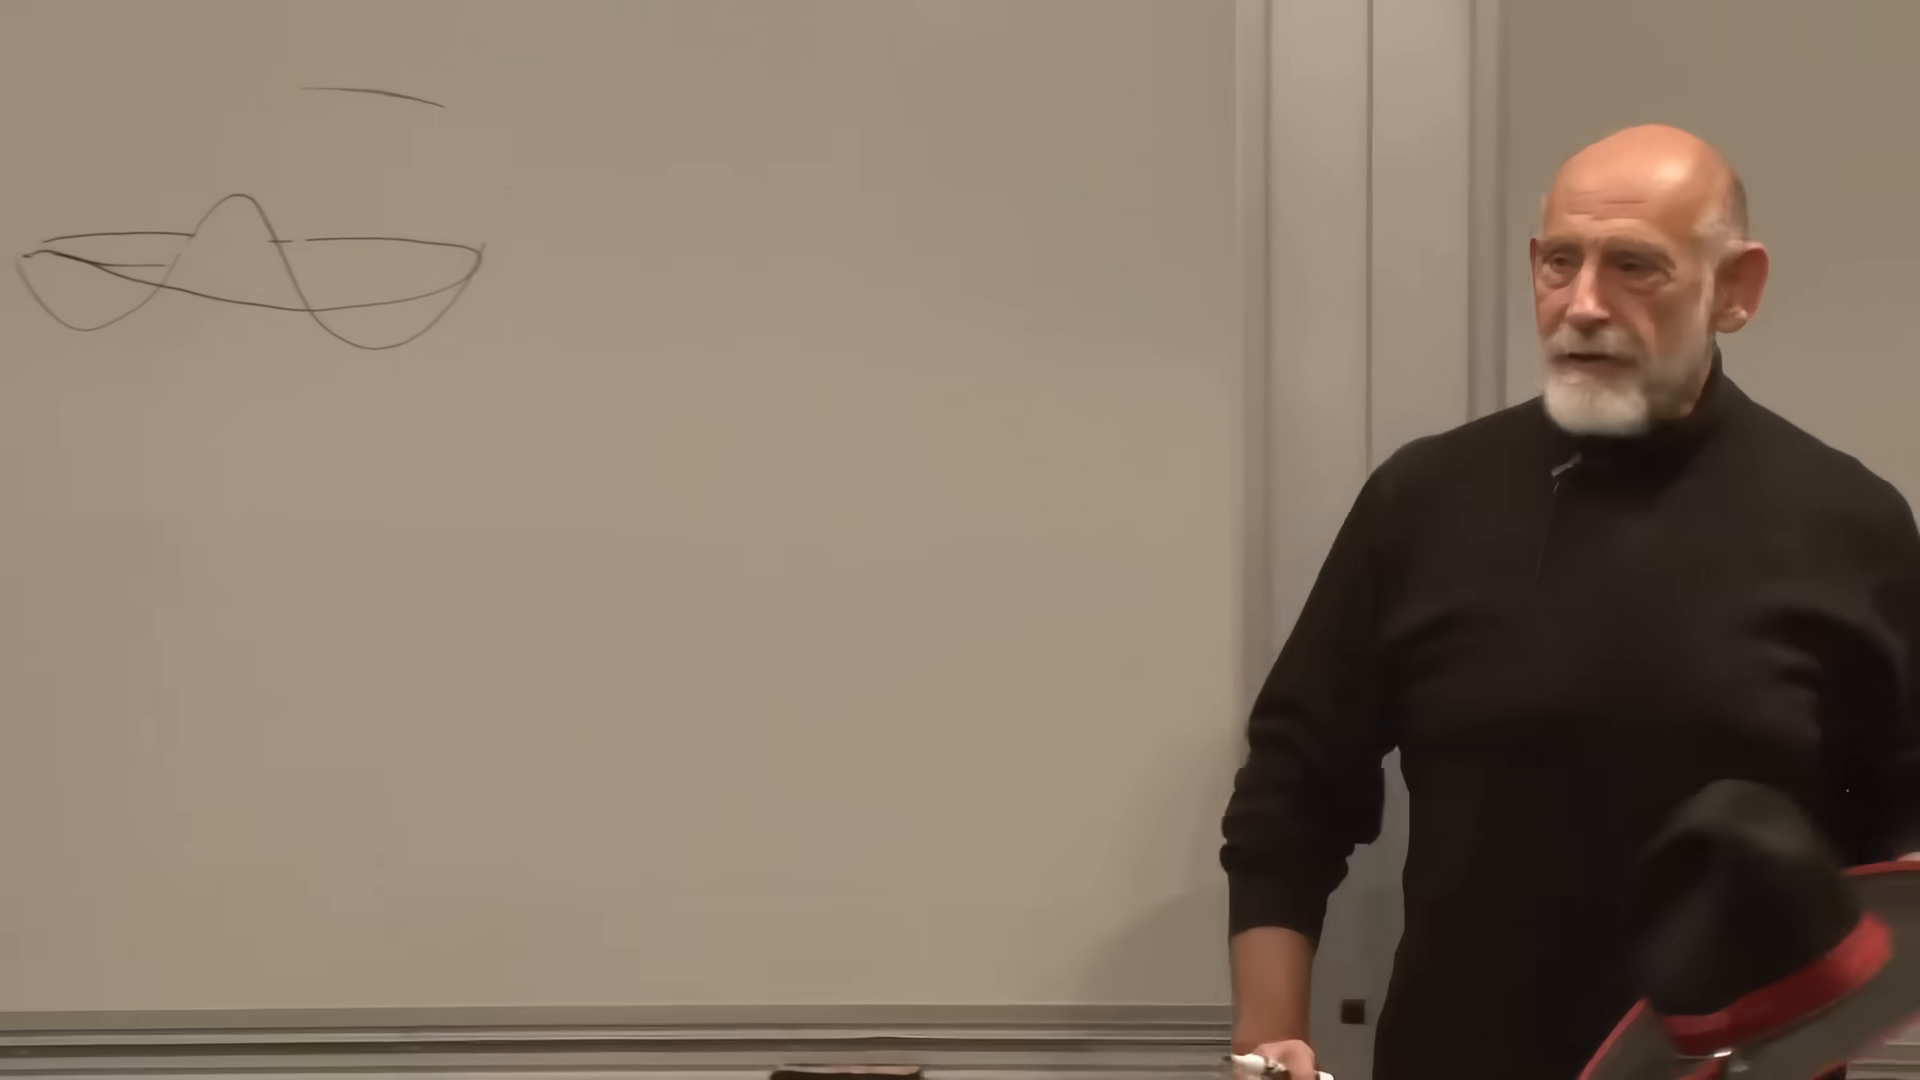
\includegraphics[width=0.95\textwidth]{lecture_144_figure_03.png}
\caption{反転した帽子型ポテンシャルの中心の峰と円形の溝。完全な板書スケッチは、幾何学の大部分を省いていた以前の切り抜きに取って代わる。}
\lectureframe{00:13:10}
\end{figure}

真空はもはや場がゼロではない。それは溝のどこかに位置しなければならない。
\begin{equation}
(\phi_1,\phi_2)
=
v(\cos\theta,\sin\theta).
\end{equation}
方程式は回転対称性を保つが、特定の真空は一つの角度 $\theta$ を選ぶ。これが自発的対称性の破れである。法則は対称であるが、選ばれた最低エネルギー状態はそうではない。

ここで質的に異なる二つの運動がある。半径方向に内側または外側へ動くとポテンシャルを登り、エネルギーを要する。溝に沿って動くと $\theta$ だけが変わり、古典的レベルではポテンシャルエネルギーを要しない。したがって、電荷のような大きな角運動量が、ごくわずかな余分なポテンシャルエネルギーと結びつきうる。

\begin{figure}[tbp]
\centering
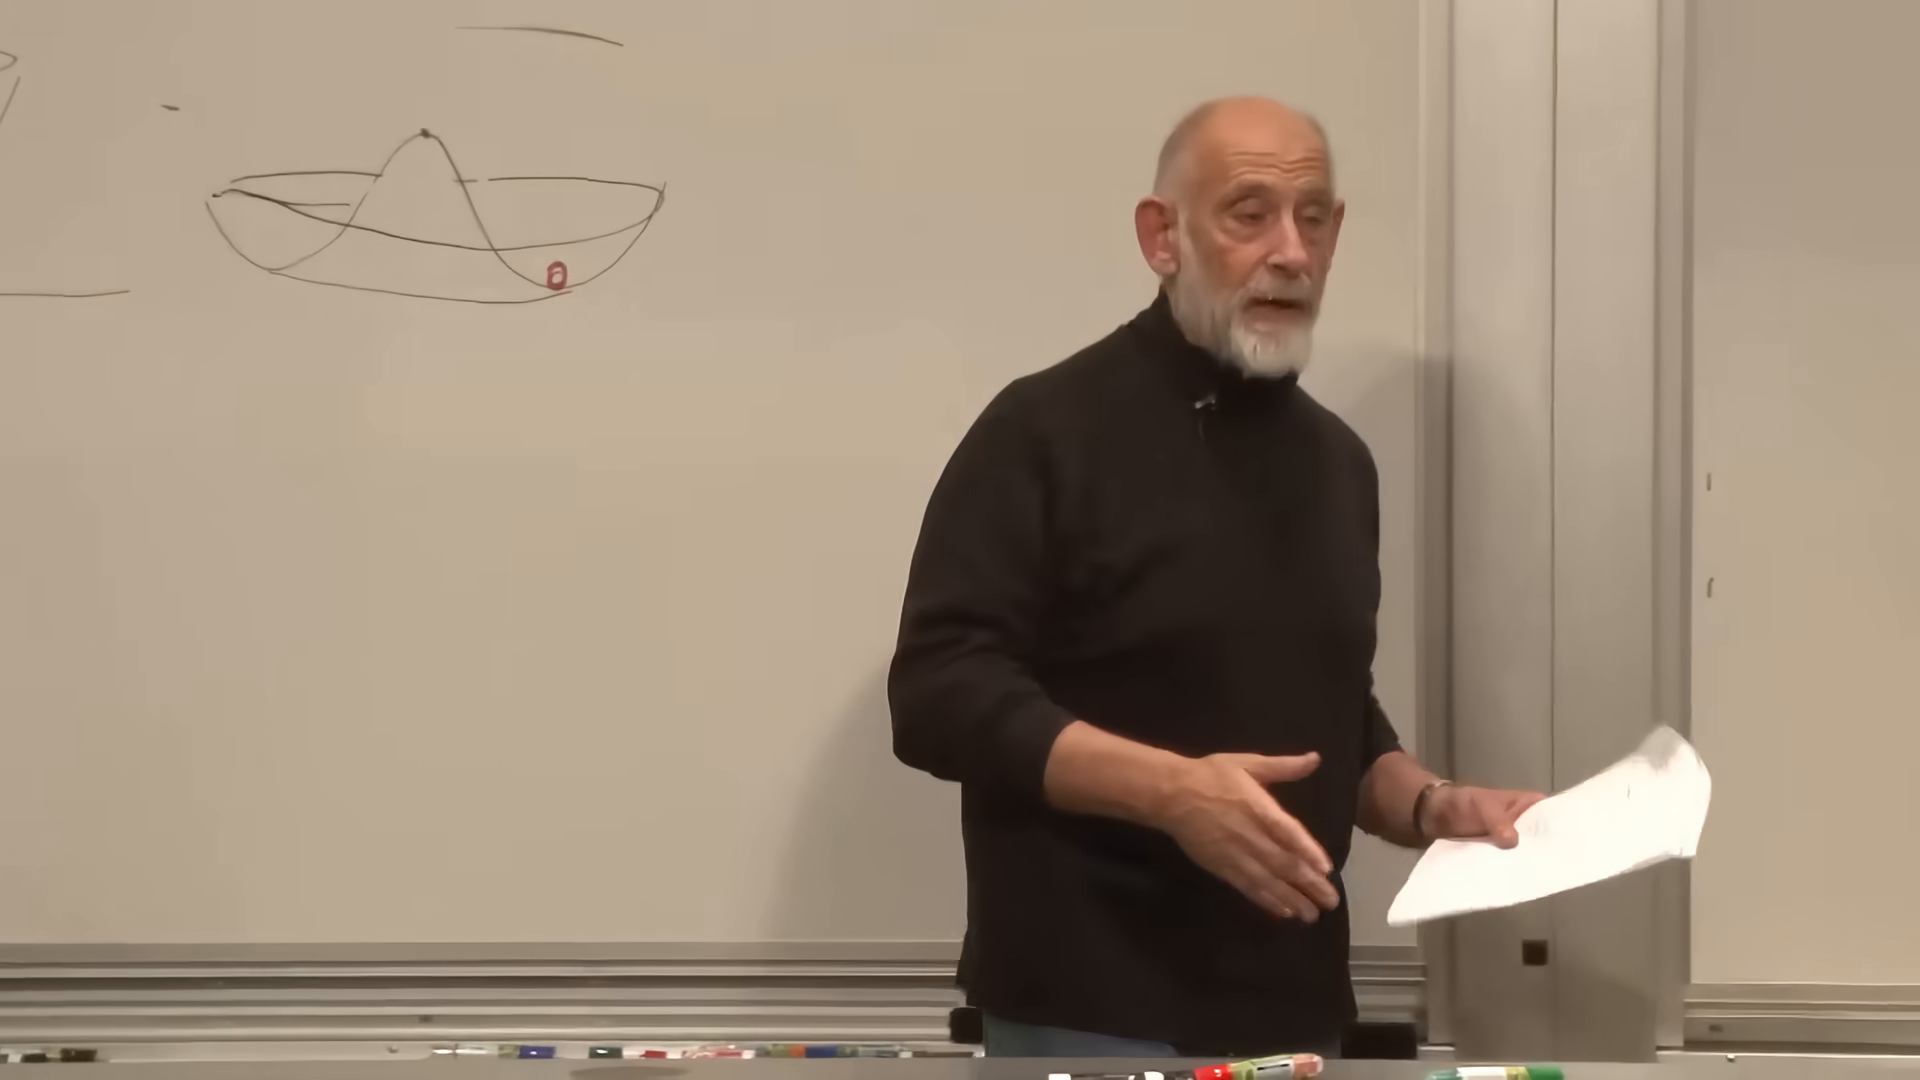
\includegraphics[width=0.95\textwidth]{lecture_144_figure_04.png}
\caption{溝の中の印された点は、等しく良好な最小値の連続的な円から選ばれた特定の真空を表す。}
\lectureframe{00:16:14}
\end{figure}

\section{不確定性が真空を凝縮体に変える}

古典的には、場を縁の一点に置き、その角速度をゼロに設定し、問題は終わったと宣言するかもしれない。量子力学はそれほど鋭い結論を禁じる。位置と運動量は
\begin{equation}
\Delta x\,\Delta p\gtrsim\frac{\hbar}{2}.
\end{equation}
を満たす。円形の溝における類似の言明は、場の角度を局在化させると、その共役な内部角運動量が不確定になるということである。講義の模式的な言葉では、
\begin{equation}
\Delta\theta\,\Delta L_{\mathrm{int}}
\gtrsim
\frac{\hbar}{2}.
\end{equation}
\editorialnote{角度演算子には技術的な微妙さがあるため、この関係は講義の不確定性議論の局所的な半古典的表現であり、大域的に厳密な演算子恒等式ではない。}

したがって、溝の一点の近くに集中した真空は、確定した内部電荷の状態ではない。それは電荷固有状態の広い重ね合わせを含む。講義はこれを操作的なテストで鋭くする。すなわち、電荷を一単位加えても、一単位除いても、状態はほとんど変わらない。模式的に
\begin{align}
\ket{\Omega}
&\sim
\sum_n c_n\ket{n},
\\
c_{n+1}
&\simeq
c_n
\quad\text{within the occupied range}.
\end{align}
と描ける。すると $n$ を一だけずらすことは、すでに存在する項のほとんどを付け替えるだけである。これが真空が \emph{凝縮体} であるという意味である。すなわち、それは関連する量子を不定数含むので、一つ多くても少なくても、観測的に異なる巨視的状態を生じない。

実際の電弱真空は通常の電荷の凝縮体ではない。もしそうなら、空の空間の電磁的振る舞いは根本的に異なるだろう。しかし超伝導体は荷電凝縮体の具体的な例を与える。したがってそれは、抽象的なメキシカンハット像と、真空がコヒーレントな量子構造を担いうるという主張との間の有用な物理的橋渡しである。

これで第一モジュールは完了する。最低エネルギー状態は場がゼロのところに座る必要はなく、量子不確定性がその状態を個々の量子の追加や除去に鈍感にしうることを学んだ。次に、どの粒子がそのような背景を必要とするのかを問う。

\section{裸の標準模型}

素粒子の質量の自然な上限の目安はプランク質量である。局在したエネルギーを十分に押し込めれば、重力を無視できなくなる。やがてその対象は普通の素粒子というよりブラックホールと見なす方がよい。数値的には、
\begin{equation}
m_{\mathrm P}
=
\sqrt{\frac{\hbar c}{G}}
\approx
2.2\times10^{-8}\,\mathrm{kg},
\end{equation}
およそ小さな塵粒の質量である。既知の素粒子は途方もなく軽い。講義で用いられたスケール推定では、それらの質量はプランク質量の約 $10^{-17}$ にしか達しない。

その観測は、より重い素粒子が存在しないことを証明するものではない。加速器は、利用可能なエネルギーで生成できるほど軽い粒子を優先的に明らかにする。したがって既知のスペクトルは、それを探索するために用いられた機械の到達範囲によって部分的に選別されている。現在の到達範囲を超えて、より重い粒子が多数存在するかもしれない。

観測される粒子はフェルミオンとボソンに分かれる。フェルミオンには電子、ミューオン、タウ、それらのニュートリノ、および六種類のクォークのフレーバーが含まれる。ボソンには光子、グルーオン、および弱い $W$ ボソンと $Z$ ボソンが含まれる。グルーオンはクォークを陽子と中性子に束縛し、その結果として通常の原子核の構造の中心をなす。

\begin{figure}[tbp]
\centering
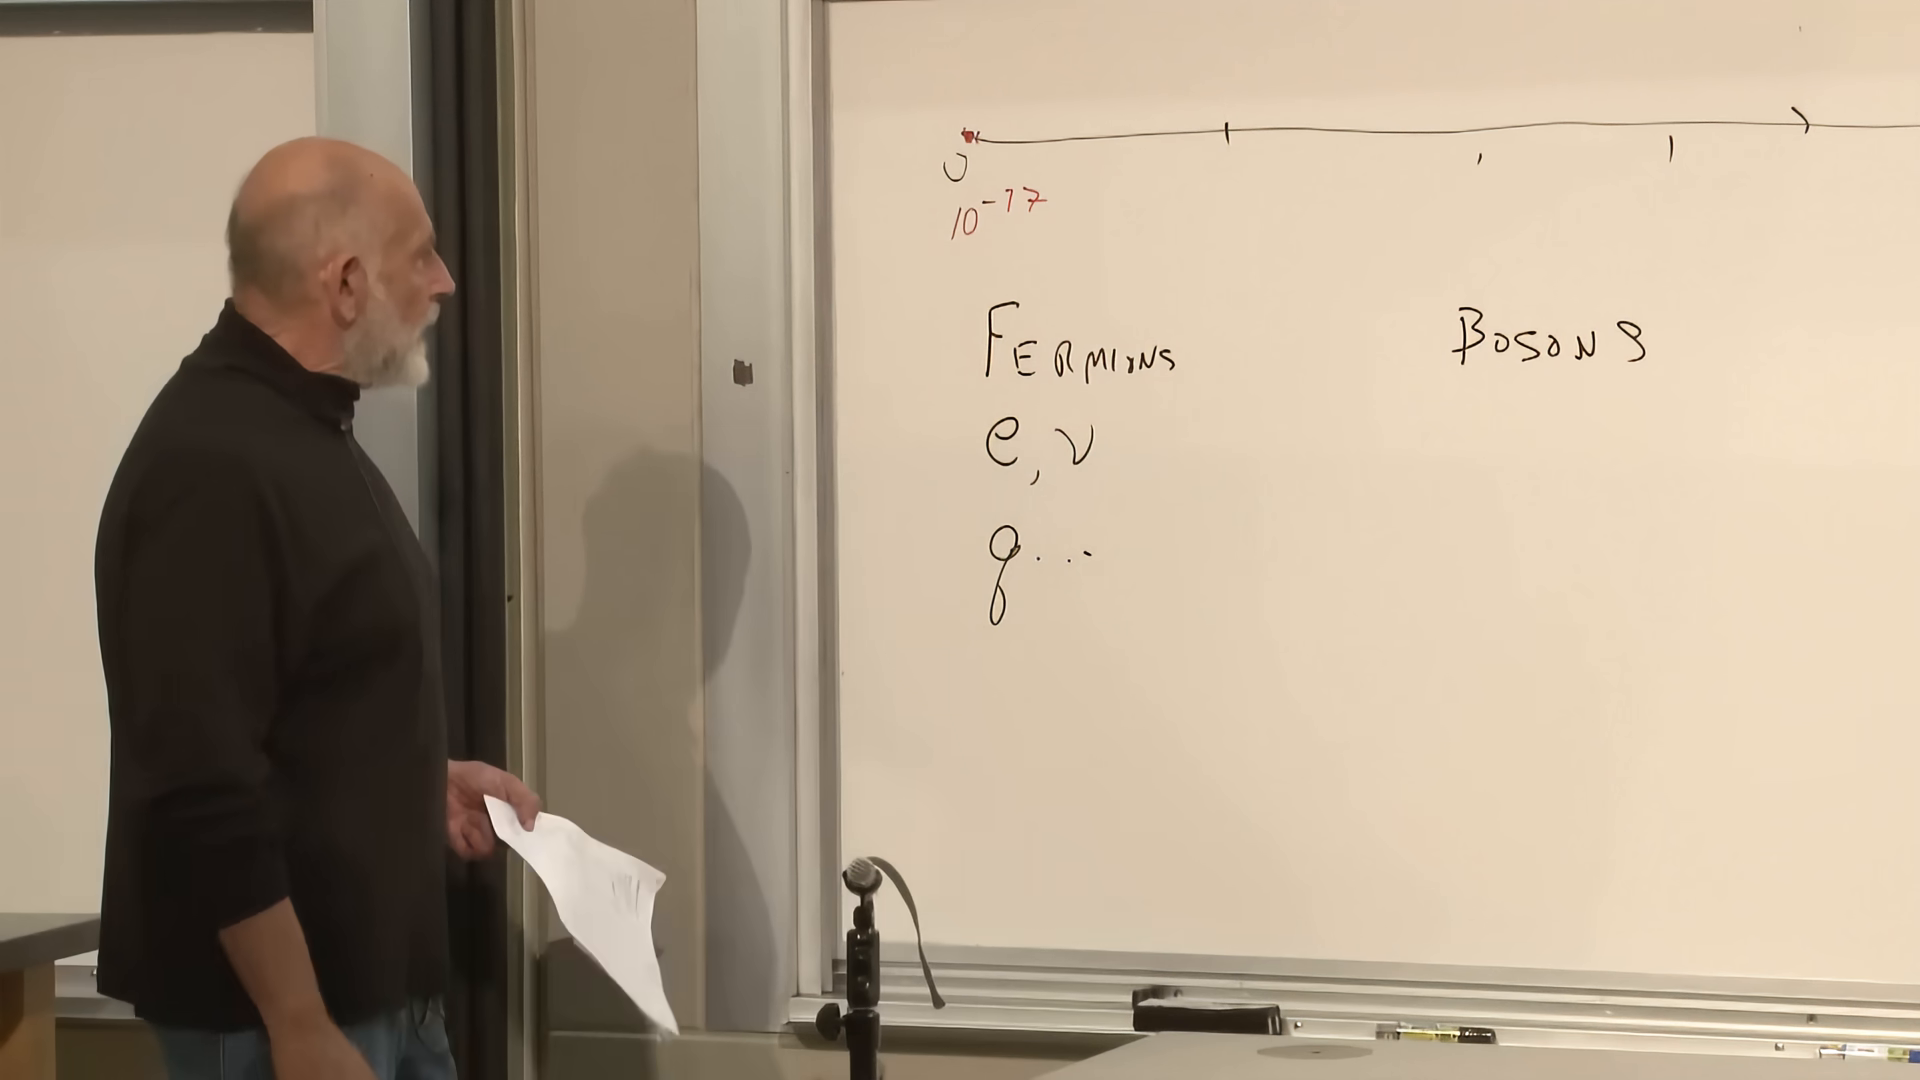
\includegraphics[width=0.95\textwidth]{lecture_144_figure_05.png}
\caption{講義における最初の標準模型の目録。フェルミオンとボソンの列の上に、巨大な質量範囲が描かれている。}
\lectureframe{00:24:22}
\end{figure}

この理論は単なる一覧ではなく、許される相互作用の集合である。電子は光子を放出してよい。
\begin{equation}
e\longrightarrow e+\gamma.
\end{equation}
クォークは電荷とカラー電荷の両方を担うので、光子またはグルーオンのいずれかを放出してよい。
\begin{equation}
q\longrightarrow q+\gamma,
\qquad
q\longrightarrow q+g.
\end{equation}
電子はグルーオンを放出できず、ニュートリノは光子もグルーオンも放出しない。適切な弱い量子数をもつフェルミオンは$Z$を通じて相互作用できる。
\begin{equation}
f\longrightarrow f+Z.
\end{equation}
$W$ボソンと荷電カレント反応もまた標準模型の一部であるが、講義では、一つの中性弱ボソンが議論を担えるように、それらを抑制している。

\begin{figure}[tbp]
\centering
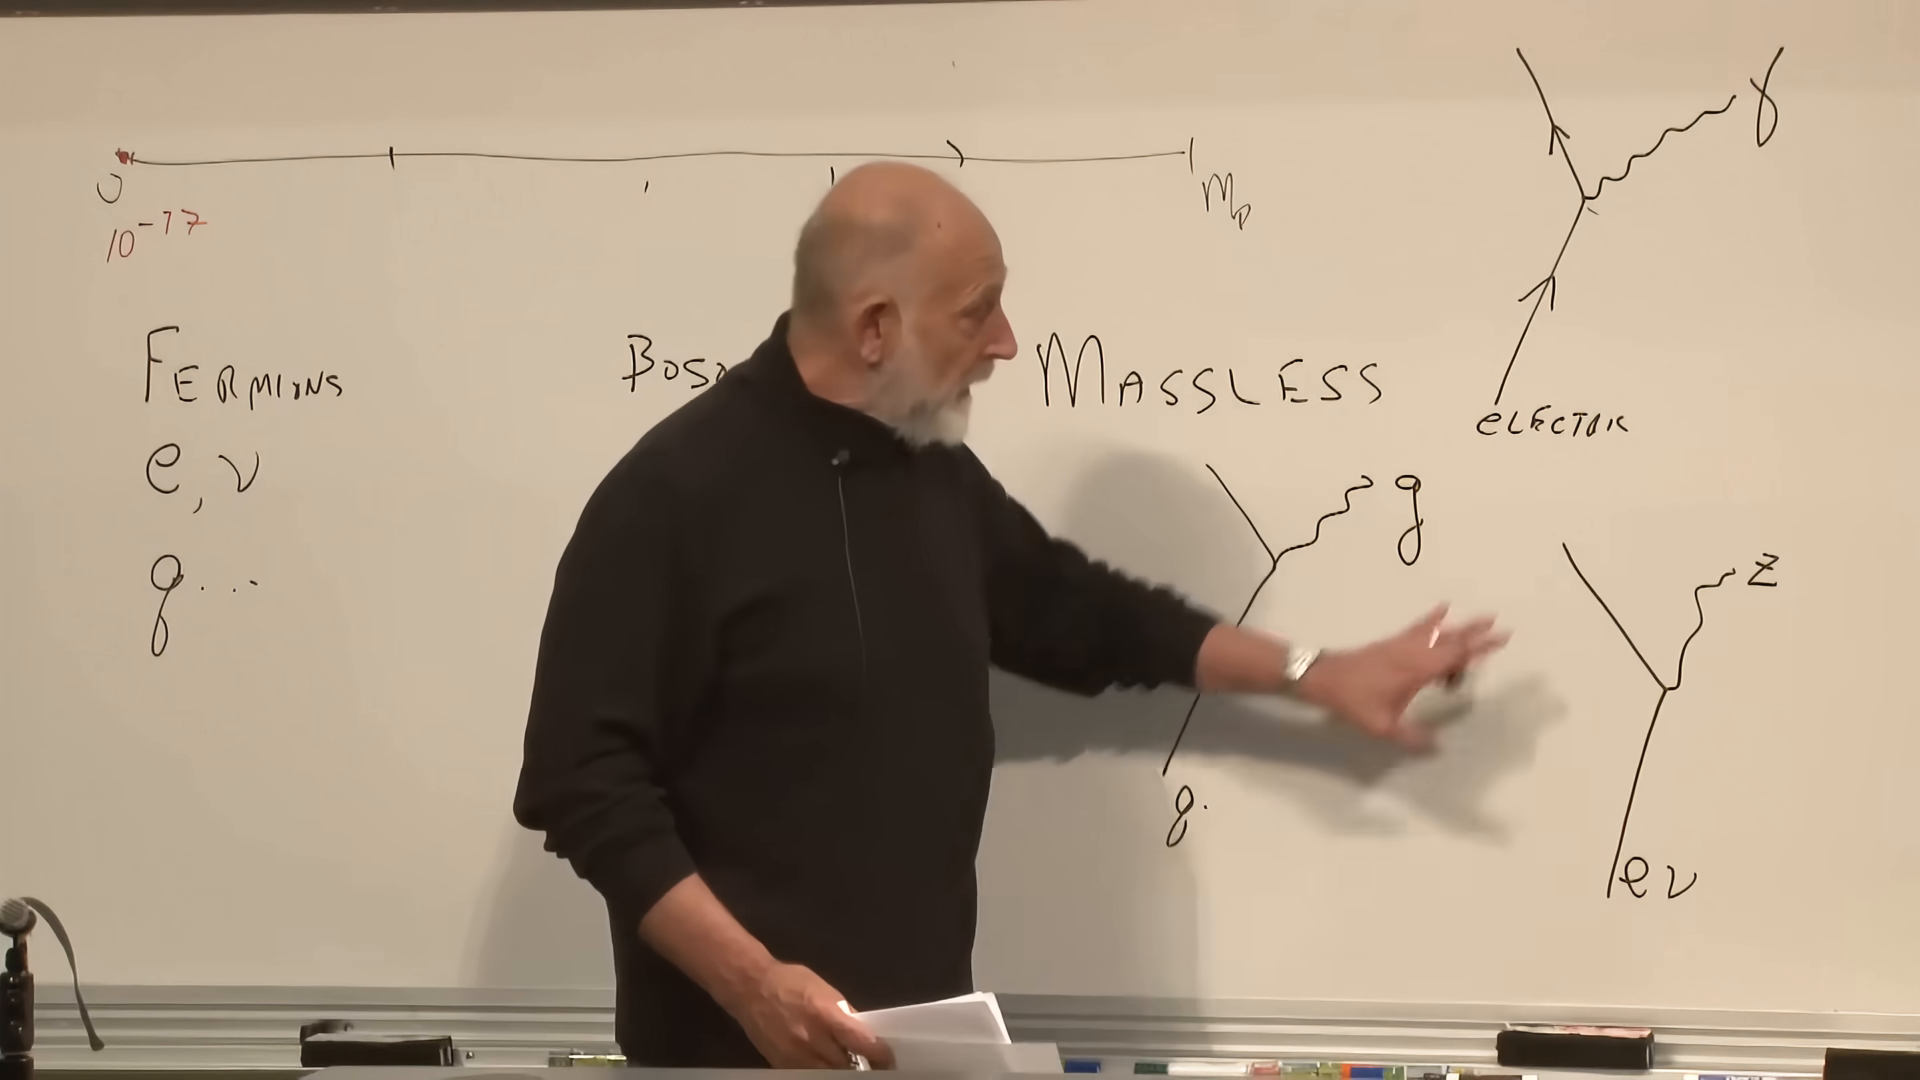
\includegraphics[width=0.95\textwidth]{lecture_144_figure_06.png}
\caption{光子、グルーオン、および$Z$放出の頂点が、``質量ゼロという語のそばに置かれている。''これらの過程は、凝縮体が導入される前の裸の理論を要約している。}
\lectureframe{00:29:20}
\end{figure}

光子は質量をもたない。同じ一般的な種類の破れていないゲージ理論では、グルーオンと弱いゲージボソンもまた質量をもたない。同様に、未修正の電弱理論は、そのゲージ対称性を保ちながらフェルミオンの質量を手で単純に挿入することはできない。一つの要素が欠けている。それを供給する前に、背景場が摩擦のように働くことなく粒子の質量を変えうる仕組みを、より単純な設定で見る必要がある。

\section{背景場はいかにして質量をずらしうるか}

水分子を電気双極子として考える。一方の端はわずかに正、他方の端はわずかに負である。空の空間では、二つの反対向きの配向はエネルギーのに等価である。講義では遊び心から、それらの配向に``ウォーター''と``スコッチ''という異なる名前を与えているが、それはそれらを異なる内部状態として追跡できるようにするためだけである。

その分子をコンデンサーの極板の間に置く。その双極子モーメントが$\bm d$であり、電場が$\bm E$であるなら、相互作用エネルギーは
\begin{equation}
U=-\bm d\mathbin{\cdot}\bm E.
\end{equation}
である。二つの整列した配向については、これは
\begin{equation}
U_{\parallel}=-dE,
\qquad
U_{\mathrm{anti}}=+dE.
\end{equation}
となる。アインシュタインの関係$E=mc^2$は、エネルギー分裂を質量分裂に変える。
\begin{equation}
m_{\mathrm{anti}}-m_{\parallel}
=
\frac{2dE}{c^{2}}.
\end{equation}
分子に何かがこすりつけられたわけではない。背景場が存在する間、一方の内部状態が他方よりも単に大きなエネルギーをもち、したがって大きな質量をもつのである。

\begin{figure}[tbp]
\centering
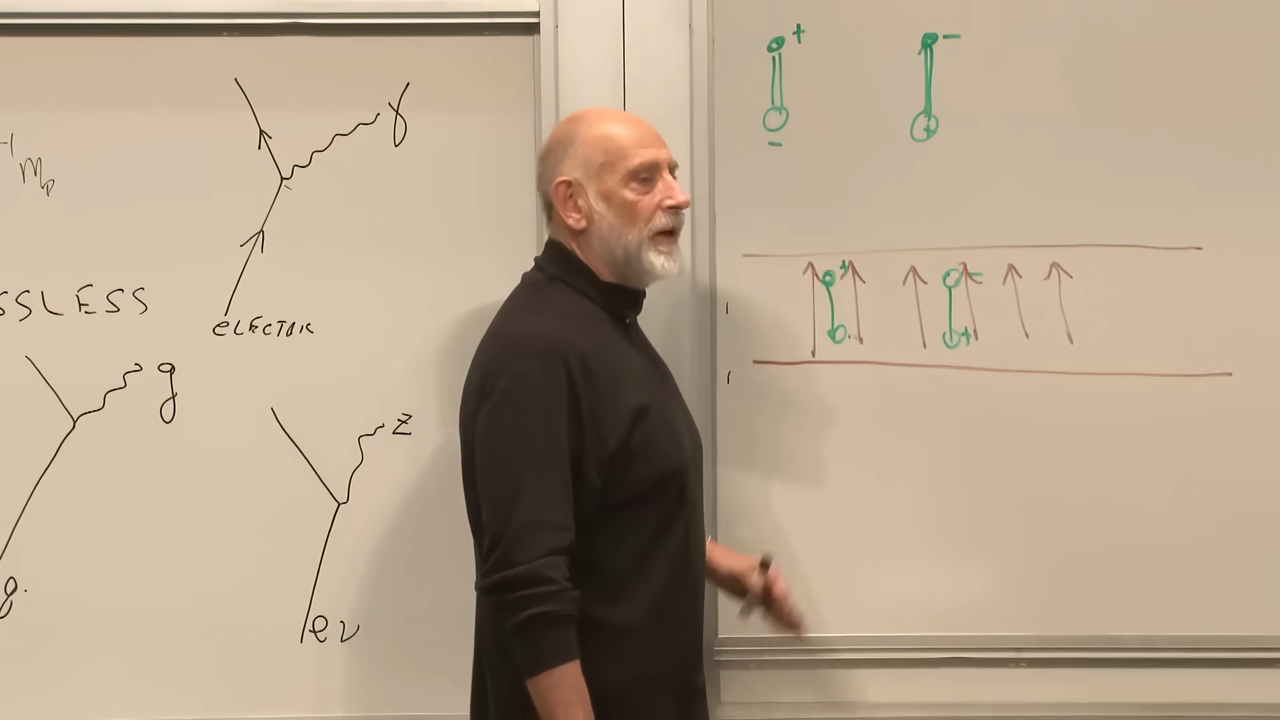
\includegraphics[width=0.95\textwidth]{lecture_144_figure_07.png}
\caption{コンデンサー場の中での反対向きの分子配向。場は、抗力をもたらすことなくそれらのエネルギーを分裂させる。}
\lectureframe{00:34:35}
\end{figure}

これは二つの誤解を招く類推を退ける。ヒッグス場は粒子が押し進まなければならない糖蜜ではなく、質量をもつ粒子は、前方に蓄積する物質によって減速される除雪車でもない。空間的に一様な場では、正味の力はまったく存在しなくてよい。効果は内部エネルギーのずれであり、摩擦でも運動量の損失でもない。

同じ例は量子の言葉で語り直すことができる。古典的な電場はコヒーレント状態であり、当面の目的のためには光子の凝縮体として記述してよい。分子はその背景へ光子を放出し、またはそこから光子を吸収してよい。一つの量子を加えたり取り除いたりすることは、高度に占有されたコヒーレント状態をほとんど変えないので、光子線は凝縮体の中で終端してよい。黒板に描かれた×印は、エネルギー保存の破れではなく、この背景への消失を表している。

\begin{figure}[tbp]
\centering
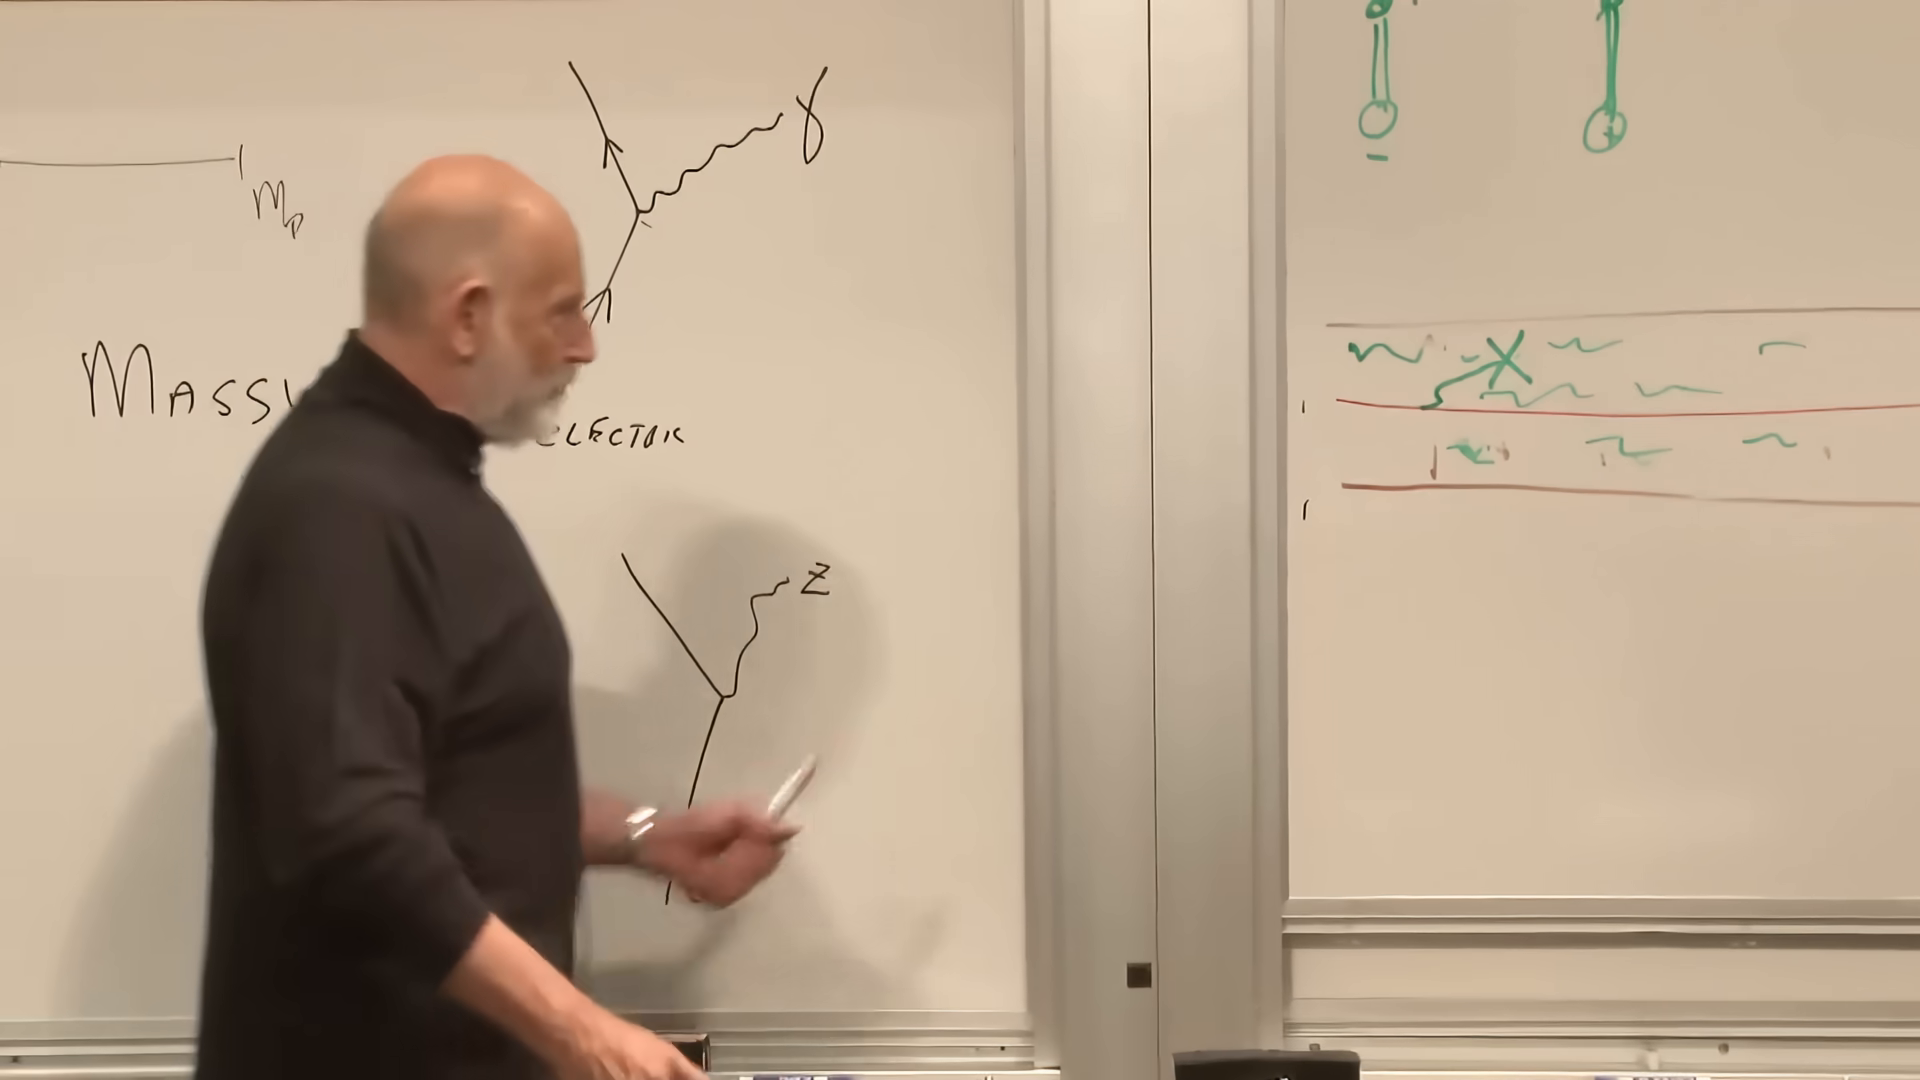
\includegraphics[width=0.95\textwidth]{lecture_144_figure_08.png}
\caption{光子凝縮体として描き直されたコンデンサー場。双極子から放出された光子は、一つの追加量子に鈍感な背景へ吸収される。}
\lectureframe{00:38:45}
\end{figure}

これが必要としていた雛形である。凝縮体が二つの内部状態の間の量子数の差を吸収できるなら、それはそれらの状態を混合できる。その結果生じる振動は質量として現れうる。

\section{なぜヒッグスはすべての質量を説明しないのか}

その雛形を適用する前に、一つの誤解を取り除かねばならない。すべての質量をもつ物体がその質量のすべてをヒッグス場から得ているというのは誤りである。

完全反射箱の中に放射を入れる。個々の光子は質量をもたないが、閉じた箱は静止系をもち、エネルギーを蓄える。その質量は次だけ増加する。
\begin{equation}
\Delta M=\frac{E_{\mathrm{radiation}}}{c^{2}}.
\end{equation}
したがって、構成要素が静止質量をもたなくても、閉じ込められた運動エネルギーと場のエネルギーから質量が生じうる。

陽子は重要な実例である。陽子はクォーク、反クォーク、グルーオンを強い相互作用をする状態で含む。陽子の質量の大部分はそれらの運動エネルギーと束縛エネルギーに由来し、少数の構成クォークのヒッグス生成質量を単に足し合わせたものに由来するのではない。講義で強調された見積もりでは、軽いクォークを質量ゼロにしても陽子の質量の変化はおよそパーセント程度にとどまる。ブラックホールはこの論理的な点をさらに際立たせる。ブラックホールが質量をもつのは、それを形成した全エネルギーによるのであって、すべての寄与がまずヒッグス場によって素粒子の静止質量に変換されたからではない。

ヒッグス機構にはより精密な役割がある。それは、基礎となるゲージ理論の整合性を保ちながら、素フェルミオンと弱いゲージボソンに質量を許す。

\section{カイラリティ：左--右混合としての質量}

まず電子に注目する。スピンは内在的な角運動量である。運動している粒子については、そのスピンの向きと運動量を比較できる。講義の幾何学的な言葉では、右巻き電子と左巻き電子はそれらの向きの関係によって区別される。質量のない粒子では、ヘリシティとカイラリティはこの議論に必要な単純な仕方で一致する。質量のある粒子では、正確な概念を区別しなければならない。

質量のある電子を繰り返し追い越すことを想像する。別の慣性系では、その運動量は反転するがスピンは反転しないので、運動の向きに付随する見かけの巻き性は反転しうる。厳密に質量のない粒子を追い越せる観測者はいない。そのような粒子は常に光速で運動する。このことが講義のヒューリスティックな主張を動機づける。質量のない電子は一つのカイラル状態にとどまるのに対し、質量のある電子は絶えず左と右を混合する。

場の理論における正確な主張は、ディラック質量項が二つのカイラル場を結合するということである。
\begin{equation}
\mathcal L_m
=
-m_e\bar e e
=
-m_e
\left(
  \bar e_L e_R
  +
  \bar e_R e_L
\right).
\end{equation}
\editorialnote{ディラック質量項は、講義の ``反転率'' という描像の標準的な数学的完成である。カイラリティの混合は質量に比例する。文字どおりの時間的割合は状態と相対論的時間の遅れに依存する。}

$m_e=0$ ならば、左場と右場は独立に伝播する。$m_e\ne0$ ならば、方程式はそれらを結合する。まさにその意味で、質量は左--右混合の強さを測る。

\section{裸の質量を禁じる保存則}

なぜ最初から混合項を単純に書いてはならないのか。弱い相互作用は $e_L$ と $e_R$ を異なる仕方で扱う。サスキンドは関連する区別に、意図的に単純な名前を与える。\emph{zilch} である。講義で用いられた規格化では、
\begin{equation}
z(e_L)=1,
\qquad
z(e_R)=0.
\end{equation}
二つのカイラリティは同じ電荷をもつが、弱い量子数は異なる。したがって直接的な遷移
\begin{equation}
e_L\longrightarrow e_R
\end{equation}
は、弱い相互作用が担う量を保存しない。破れていない理論では、裸の質量項は禁じられている。

\editorialnote{``Zilch'' は教育的な略記である。標準模型では、左巻きフェルミオンと右巻きフェルミオンは異なる $SU(2)_L\times U(1)_Y$ 表現に属するので、直接的なディラック質量項はゲージ不変ではない。講義の割り当て $1$ と $0$ は、完全な電弱電荷表を再現することなくこの違いを符号化している。}

黒板はこの障害を連鎖として提示する。右巻き電子は、何か他のものが zilch の差を持ち去らない限り、左巻きになることができない。同じ障害がクォーク、ミューオン、タウにも当てはまり、欠けている場が与えられれば、その強さは種に依存する。

\begin{figure}[tbp]
\centering
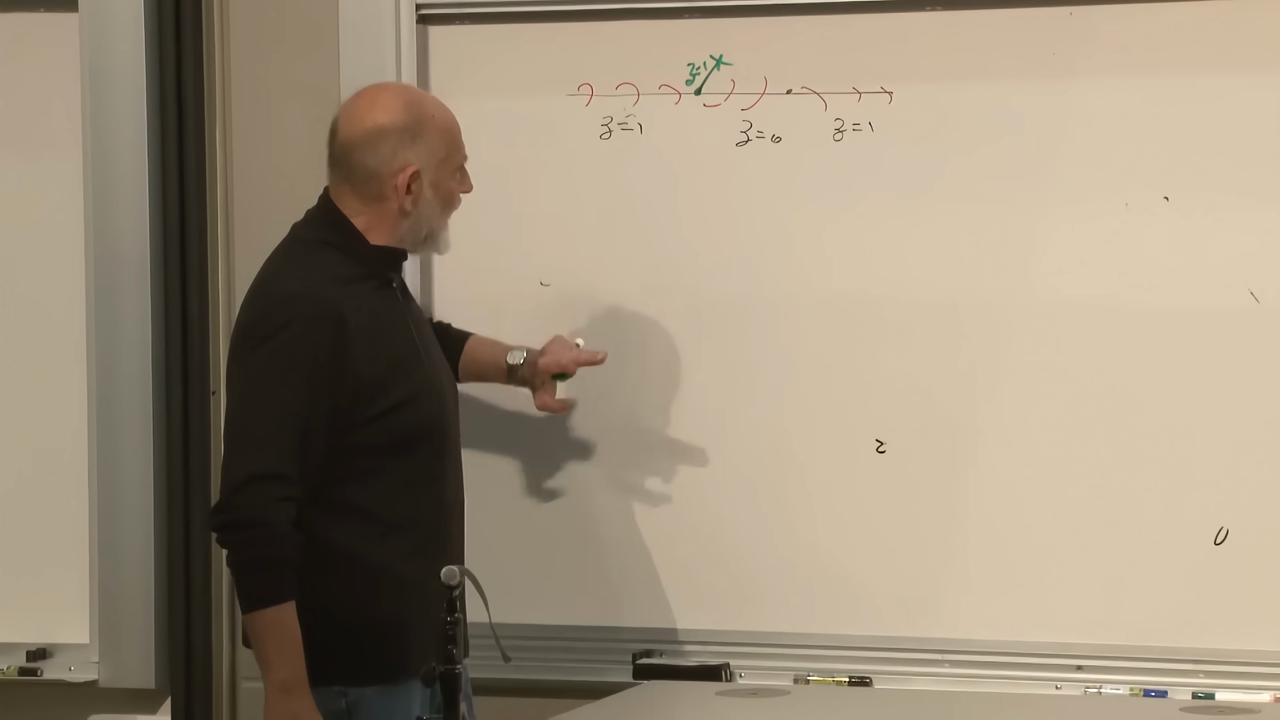
\includegraphics[width=0.95\textwidth]{lecture_144_figure_09.png}
\caption{黒板上のカイラルな順序：緑の十字に挿入された凝縮体の量子が、右巻き伝播と左巻き伝播の間で zilch のラベルを変えることを可能にする。}
\lectureframe{00:50:15}
\end{figure}

\section{``Ziggs''凝縮体とフェルミオン質量}

その量子がまさに欠けている弱い量子数を持つ場を導入する。物理的なヒッグス粒子との早すぎる混同を避けるため、講義ではその関連する量子を\emph{ジグス}と呼ぶ。ジグス場がメキシカンハット型ポテンシャルを持ち、その真空が凝縮体であると仮定する。すると、左巻きの電子はジグス量子を放出して右巻きになり、
\begin{equation}
e_L\longrightarrow e_R+\text{Ziggs},
\end{equation}
あるいは右巻きの電子はジグス量子を吸収して左巻きになる。
\begin{equation}
e_R+\text{Ziggs}\longrightarrow e_L.
\end{equation}
凝縮体はその巨視的状態を変えることなく量子数の差を吸収または供給する。空の非破れ真空では禁じられていたことが、対称性の破れた真空では許されるようになる。

放出と吸収の繰り返しが$e_L$と$e_R$を混合させる。したがって電子は質量を持つ粒子として伝播する。同じ機構が荷電レプトンとクォークにも当てはまる。それぞれの種は凝縮体との独自の結合を持つため、反転の強さ、ひいては質量は種ごとに異なりうる。

現代的な記法では、ゲージ不変な相互作用は湯川結合である。ヒッグス場が真空期待値$v$を獲得した後、それは
\begin{equation}
\mathcal L_Y
\supset
-\frac{y_f}{\sqrt{2}}
(v+h)\bar f f,
\end{equation}
を生み、したがって
\begin{equation}
m_f=\frac{y_fv}{\sqrt{2}},
\qquad
g_{hff}=\frac{y_f}{\sqrt{2}}
=
\frac{m_f}{v}.
\end{equation}
\editorialnote{これらの式は、講義の凝縮体結合の議論の背後にある標準的な電弱記法を与える。また、同じ結合がフェルミオン質量とそのフェルミオンへのヒッグス崩壊の両方を制御する理由も明示する。}

講義ではこれをカイラル対称性の自発的破れとして説明している。それはこの例のレベルで左右--の話を捉えている。より正確には、ヒッグス期待値は電弱ゲージ対称性を電磁部分群へ破り、その後ユカワ相互作用がフェルミオン質量項になる。

\section{弱いボソンはいかにして質量を獲得するか}

凝縮体は弱いゲージボソンも変える。ジグス励起は$Z$ボソンを放出でき、逆に$Z$は適切な凝縮体に支えられた励起に変わり、また戻ることができる。したがって$Z$は、ヒッグス場の角度セクターと混合する真空中を伝播する。その結果は、質量のないベクトルボソンが持たない縦偏極を持つ、質量のあるベクトルボソンである。

\begin{figure}[tbp]
\centering
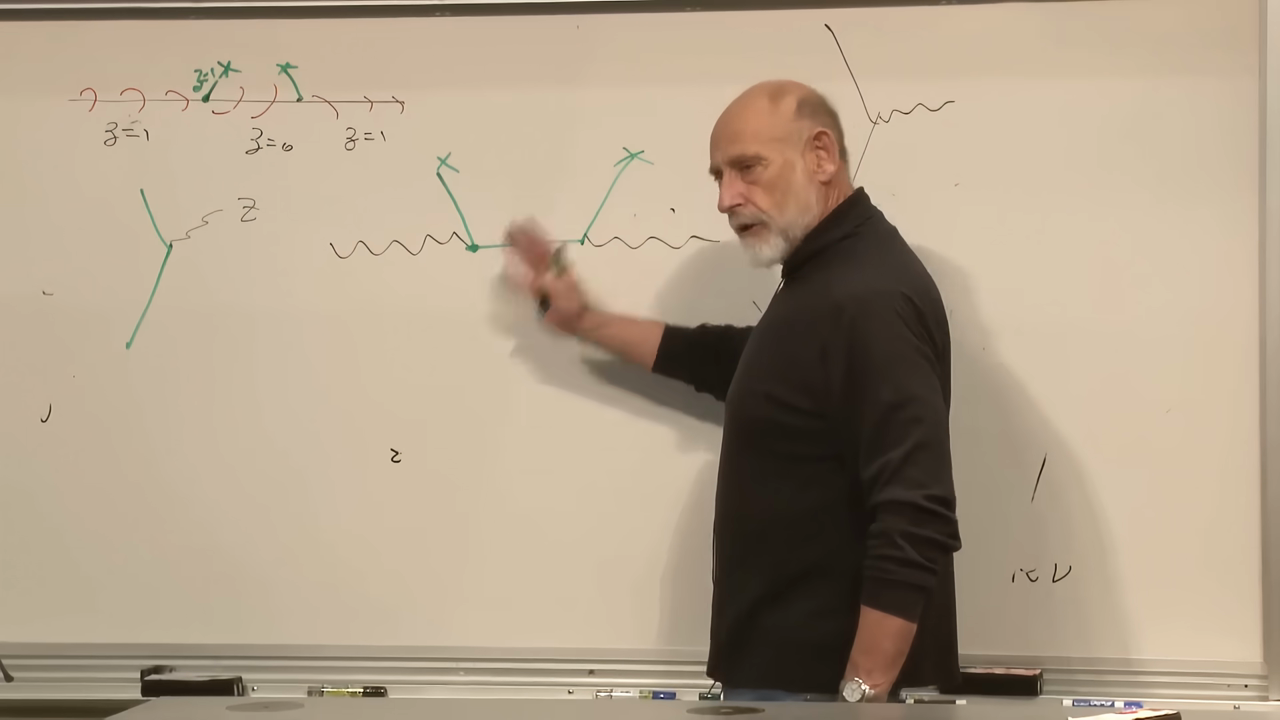
\includegraphics[width=0.95\textwidth]{lecture_144_figure_10.png}
\caption{弱いボソン機構の完成した板書の順序：カイラル連鎖は上に残り、一方$Z$は下の凝縮体に支えられたセクターと量子数を交換する。}
\lectureframe{00:53:40}
\end{figure}

これがゲージボソンの形でのブロート--エングレールト--ヒッグス現象である。完全な標準模型では、$W$ボソンと$Z$の両方が質量を獲得する一方、元の中性ゲージ場のある組み合わせは質量のない光子として残る。もし真空が代わりに通常の電磁ゲージ対称性を破っていたなら、光子は質量を持ったであろう。超伝導体の内部で実効的にそうなるように。そのとき空虚な空間は、まったく異なる長距離電磁的振る舞いを持つことになる。

弱いボソンは、物理的なヒッグス粒子が単離されるずっと前に、すでにこの機構に対する強い証拠を与えていた。それらの質量と相互作用は、電弱対称性が必要な仕方で破れていることを示していた。だからこそ講義は、緩い操作的意味で、``ジグス''セクターはすでに知られていたと言えるのである。欠けていた実験的対象は、独立な動径方向の振動であった。

\editorialnote{1980前後のSLACでの発見への講義の即興的な言及は、いくつかの出来事を圧縮している。中性弱電流は1973に観測され、SLACでのパリティを破る電子散乱は1970年代後半に報告され、$W$ボソンと$Z$ボソンは1983にCERNで直接発見された。物理的な要点は、電弱対称性の破れが以前に実験的に確認されていたことである。}

\section{ヒッグス粒子とは実際には何か}

メキシカンハットに戻る。谷に沿った運動は角度を変えるが半径は変えない。その角度セクターが、質量を持つ弱いボソンに吸収されるモードを与える。物理的なヒッグス粒子はもう一方の運動である。ポテンシャルの壁を内側へ外側へと振動することである。

場を模式的に次のように書く。
\begin{equation}
\Phi(x)
=
\frac{v+h(x)}{\sqrt{2}}
\exp\!\left(
  \frac{i\theta(x)}{v}
\right).
\end{equation}
変数$\theta$は谷に沿った運動を記述する。変数$h$は半径を変える。ゲージ理論では、適切な角度自由度は質量のある弱いボソンの縦成分になり、一方$h$は伝播するスカラー粒子、すなわちヒッグス粒子として残る。

\begin{figure}[tbp]
\centering
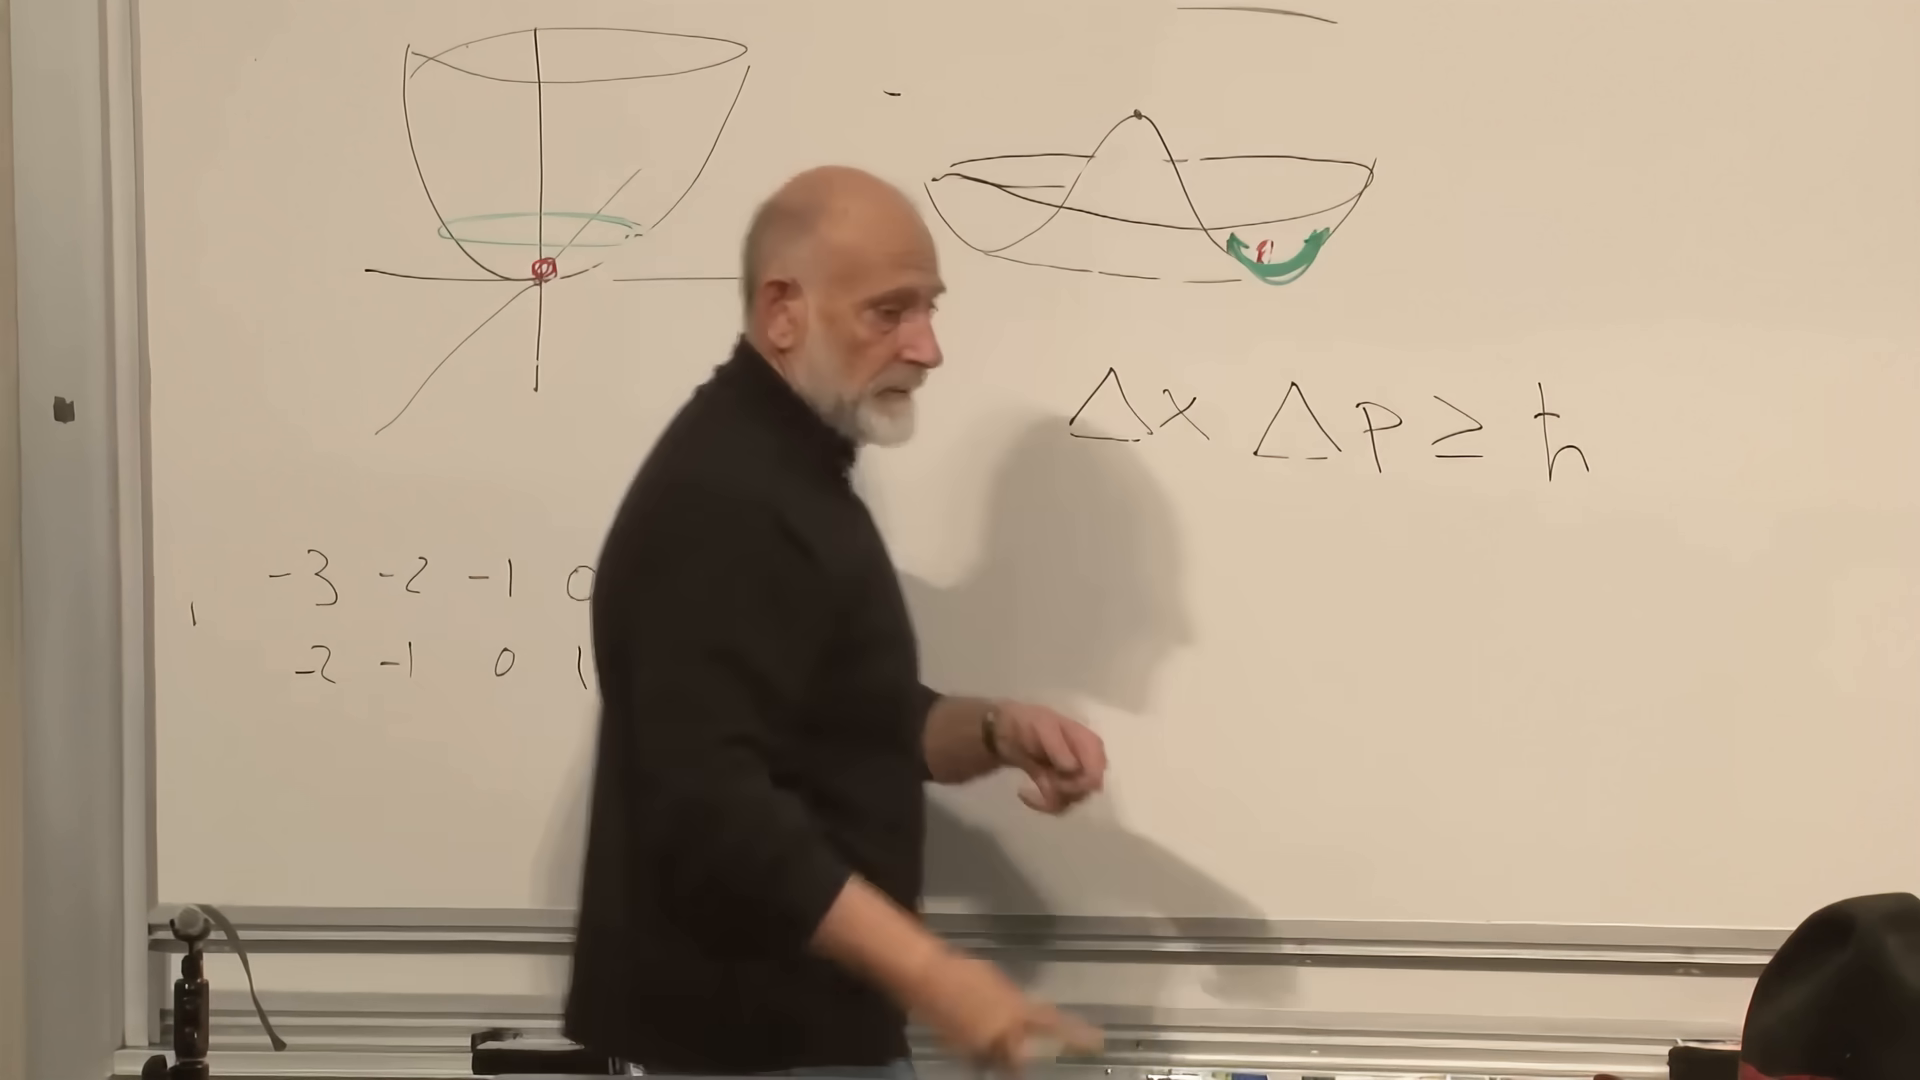
\includegraphics[width=0.95\textwidth]{lecture_144_figure_11.png}
\caption{両方のポテンシャルが再び板書され、メキシカンハットの谷に動径方向の変位が記されている。この出入りの振動が物理的なヒッグスモードである。}
\lectureframe{00:56:30}
\end{figure}

等価な多粒子描像がある。真空は凝縮体であり、動径振動は凝縮体の密度を変える。したがってヒッグス粒子はその量子媒質中の圧縮波のようなものである。この類推は、その波が安定でなければならないと推論しない限り有用である。通常の音波は減衰しうるし、ヒッグス励起も同様に減衰しうる。

この区別は、ヒッグス粒子の発見がこの機構の最初の証拠ではなく最後の欠けたピースであった理由を説明する。破れた真空と質量をもつ弱ボソンはすでに間接的に見えていた。動径密度波は粒子として生成され、その崩壊生成物を通じて同定されなければならなかった。

\section{崩壊、生成、そして重いフェルミオンの利点}

ヒッグスはフェルミオンとの結合がそのフェルミオンの質量に比例する。それはフェルミオン-反フェルミオン対へ崩壊しうる。
\begin{equation}
H\longrightarrow f+\bar f,
\end{equation}
そして同じ図は逆向きに読んで生成とすることができる。
\begin{equation}
f+\bar f\longrightarrow H.
\end{equation}
したがって電子-陽電子対消滅は原理的には可能である。しかし歴史的には、初期の衝突型加速器はまずヒッグスを作るのに十分なエネルギーを欠いており、後の機械は電子のユカワ結合が極端に小さいという、より根本的な問題に直面した。軽いクォークの対消滅も同様に弱い。

\begin{figure}[tbp]
\centering
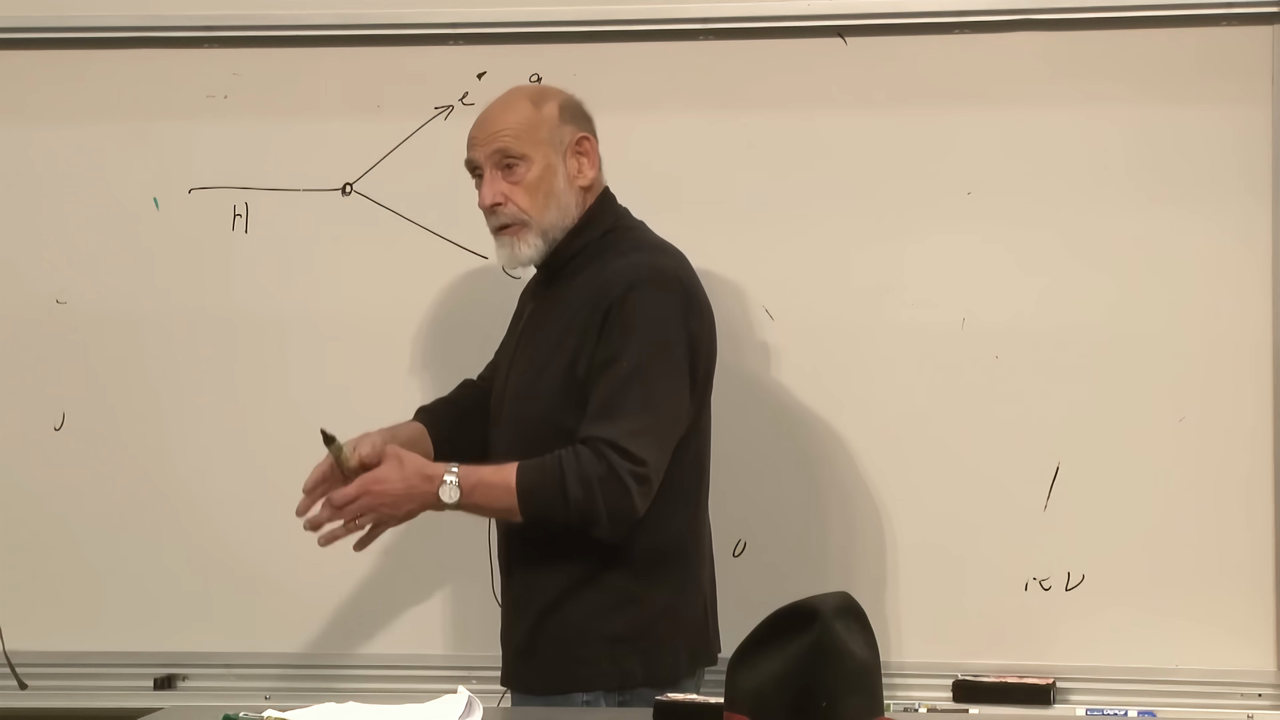
\includegraphics[width=0.95\textwidth]{lecture_144_figure_12.png}
\caption{板書されたヒッグス崩壊の頂点。矢印を逆向きに読むとフェルミオン-反フェルミオン融合によるヒッグス生成となる。}
\lectureframe{00:59:40}
\end{figure}

フェルミオンが重いほど、そのユカワ結合は大きい。これがトップクォークを際立たせる。その質量は約$173\,\mathrm{GeV}$、すなわちおよそ$180$個の陽子質量である。講義では約$170$個の陽子質量という概数を用いている。しかし質量が$125\,\mathrm{GeV}$付近のヒッグスは、オンシェルの$t\bar t$対へ崩壊するには軽すぎる。
\begin{equation}
m_H<2m_t.
\end{equation}
また、有用なトップクォークのビームを作ることもできない。トップは長寿命のビーム粒子へハドロン化する前に崩壊する。

量子力学は両方の障害を回避する方法を与える。二つのグルーオンは仮想トップクォークループを経て揺らぎ、ヒッグスとして出てくることができる。
\begin{equation}
g+g\longrightarrow H.
\end{equation}
仮想トップの線は、実トップ対生成を支配するであろうオンシェル閾値を満たす必要はない。陽子はグルーオンで満たされているので、大型ハドロン衝突型加速器における高エネルギー陽子-陽子衝突は、必要なグルーオン対の強力な源を提供する。

\begin{figure}[tbp]
\centering
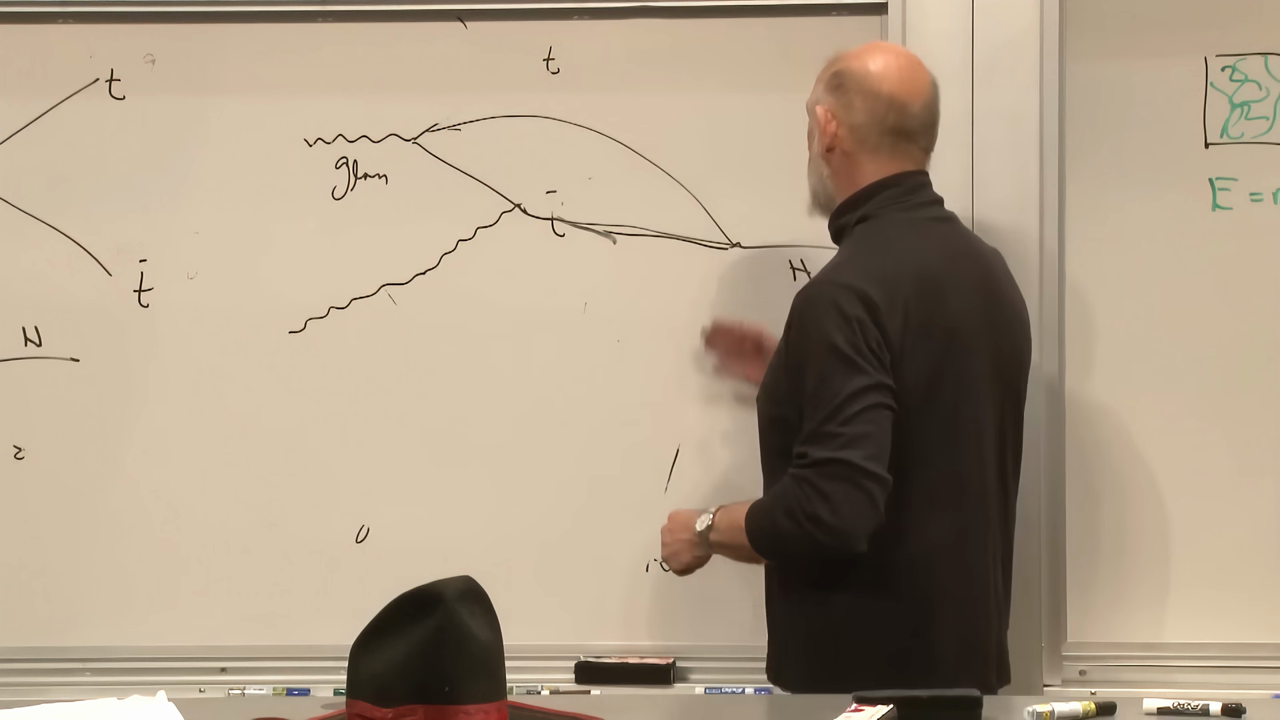
\includegraphics[width=0.95\textwidth]{lecture_144_figure_13.png}
\caption{仮想トップループを通じたグルーオン融合。衝突する陽子から取られた二つのグルーオンがループで出会い、ヒッグスを生成する。}
\lectureframe{01:06:35}
\end{figure}

これが、陽子の破片の複雑さにもかかわらず、陽子衝突型加速器が決定的なヒッグス工場となった理由である。陽子は一つの素粒子としてヒッグスと結合するのではない。そのグルーオン構成要素が、重いトップ結合に支配されたループを通じてヒッグスを生成する。

\section{2012年の粒子とその二光子テスト}

2012年に報告された粒子は、
\begin{equation}
m_H\simeq125\,\mathrm{GeV}.
\end{equation}
付近の質量をもっていた。講義の便宜的な比較では、それはおよそ$127$個の陽子質量である。その発見は、最小標準模型が要求する粒子のリストを完成させた。残る問題は、その定量的性質が正確に標準模型の性質であるかどうかであった。

トップループの論理は逆に使うことができる。ヒッグスはループ中の仮想荷電粒子と結合し、そのループは二つの光子を放出しうる。
\begin{equation}
H\longrightarrow\gamma+\gamma.
\end{equation}
この崩壊は稀であるが、光子はハドロン衝突型加速器において例外的にきれいな物体である。したがって、その不変質量分布における狭い超過は、より一般的な崩壊が実験的に乱雑である場合でもヒッグスを明らかにしうる。

\begin{figure}[tbp]
\centering
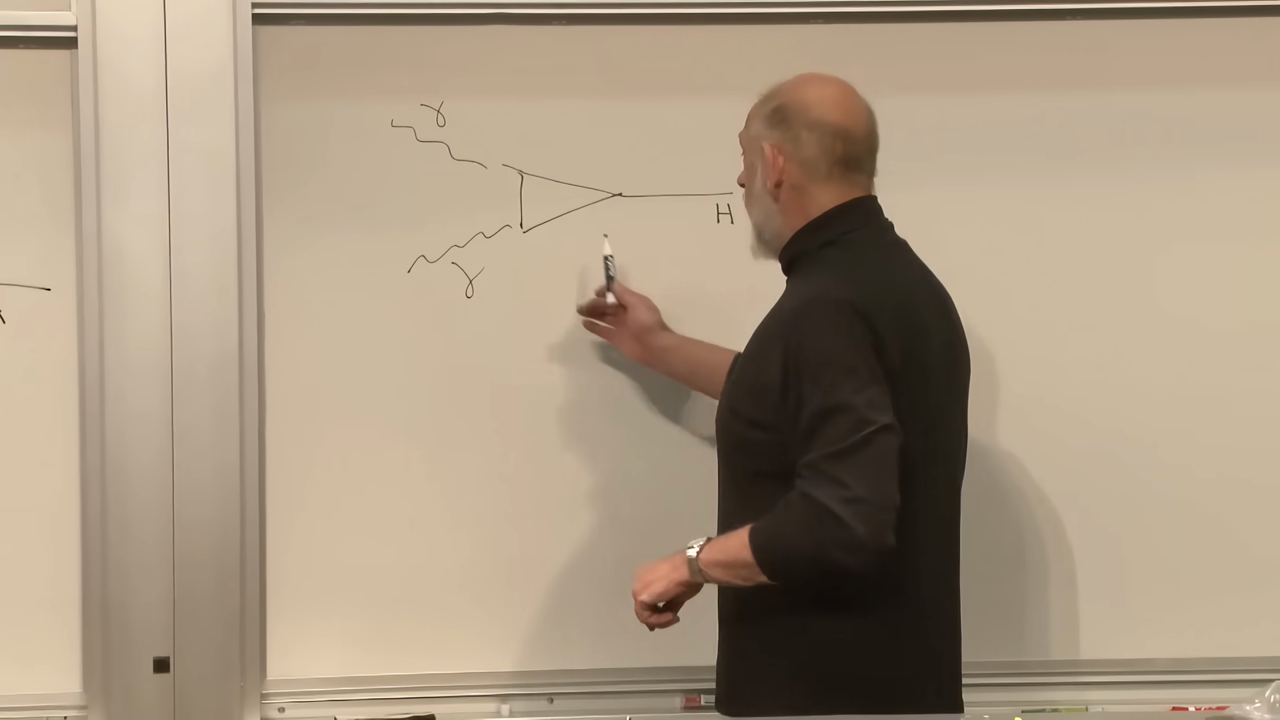
\includegraphics[width=0.95\textwidth]{lecture_144_figure_14.png}
\caption{板書の右側にある二光子の三角形は、左側の先のグルーオン融合ループと対をなしている。この二つの過程は同じループレベルの論理を反対方向から探る。}
\lectureframe{01:09:00}
\end{figure}

講義当時、報告されていた二光子率は、最も単純な標準模型の予想のおよそ1.5倍に見えたが、有意性はわずか約2標準偏差にすぎなかった。そのような揺らぎは、それ自体では証拠とはならなかった。しかし、もしそれが持続していれば、ループに追加の荷電粒子が存在することを示唆し得た。おそらく超対称性や標準模型の別の拡張に関連する粒子であろう。

その記述は2012という歴史的時点に属するものである。それは、実験家たちが次に何を注視するよう言われていたかを記録したものであり、現在の異常の主張ではない。発見そのものは、すでに弱ボソンのデータによって支持されていた枠組みの、大部分は確認であった。科学的により鋭い検証は崩壊率であった。新しいスカラーは、ヒッグス機構が予言する質量依存のパターンで各粒子と結合するのか、ということであった。

\section{聴衆からの質問}

\begin{classroomqa}
\audiencequestion{あるフェルミオンが別のフェルミオンより速く左右振動し、したがって異なる質量をもつのは、何によって決まるのか。\lecturetimestamp{01:12:00}}
\lecturerresponse{各フェルミオン種は、ヒッグス凝縮体との独自の結合をもつ。より強い結合は、より強い左--右混合とより大きな質量を生み出す。同じ結合が、物理的ヒッグスがそのフェルミオンへどれほど強く崩壊するかを決めており、それゆえ一般により重いフェルミオンほどより強く結合する。標準模型はこれらの湯川結合をパラメータ化するが、その際立った階層性を説明しない。電子は小さな結合をもち、トップクォークは大きな結合をもつと言うことは、正確な記述ではあるが、まだより深い導出ではない。}
\end{classroomqa}

\begin{classroomqa}
\audiencequestion{真空中のヒッグス場の大きさは分かっているのですか。\lecturetimestamp{01:13:36}}
\lecturerresponse{はい。ここで用いている規約では、真空期待値はおよそ$240\,\mathrm{GeV}$であり、より正確な標準的な値はおよそ$246\,\mathrm{GeV}$である。それは、場の原点からの動径方向の変位として描くことも、凝縮体の密度として描くこともできる。物理的ヒッグス量子は、その値の小さな動径方向の振動であり、等価に、凝縮体の局所的な密度揺らぎである。}
\end{classroomqa}

\begin{classroomqa}
\audiencequestion{ヒッグス場のゼロでない真空値は、空の空間のエネルギー密度を意味するのですか。\lecturetimestamp{01:14:12}}
\lecturerresponse{はい。ヒッグスポテンシャルは真空エネルギーに寄与し、量子場理論の他の多くの部門も同様に寄与する。観測される正味の真空エネルギーは、それらの寄与の自然な大きさに比べて極めて小さいので、それらはほぼ相殺しなければならない。その相殺を説明する受け入れられた理論はない。これが宇宙定数問題であり、基礎物理学における最も深い未解決問題の一つである。}
\end{classroomqa}

\section{この構成が成し遂げたこと}

この論理は、今や粘っこいエーテルを持ち出すことなく、初めから終わりまで読み通すことができる。量子化された内部回転が電荷の模型を与える。椀をメキシカンハットに変えると、場にゼロでない真空値が与えられる。不確定性原理は、鋭く選ばれた古典的真空を、個々の量子に鈍感な凝縮体へと変える。そうして凝縮体は、左手系と右手系のフェルミオン間の弱い量子数の差を担うことができ、それによって両者の混合、ひいては質量を可能にする。またそれは、$W$と$Z$が質量をもつベクトルボソンとして伝播することを可能にし、一方で光子は質量をもたないままでいられる縦モードを与える。

物理的ヒッグスボソンは、この再編成の後に残る動径方向の振動である。それは``質量そのもの''ではなく、陽子の質量の大部分の原因でもない。それは、対称性の破れを起こした場の観測可能な密度波である。その結合は、その場によって生成された質量を記憶しており、それゆえ重い粒子がその生成と崩壊を支配する。グルーオン融合ループ、二光子チャネル、そして真空エネルギーについての聴衆の最後の質問は、したがって別々の珍しい話ではない。それらは、同じ非自明な真空の帰結であり、検証であり、未完成の含意なのである。
